\documentclass{beamer}
%\usetheme{Ilmenau}
%\usecolortheme{beaver}

\usepackage[slovak,american]{babel}
\usepackage[utf8]{inputenc}
\usepackage{graphicx}
\usepackage{adjustbox}
 \usepackage{xcolor}
 
 \newsavebox\MBox
\newcommand\Cline[2][red]{{\sbox\MBox{$#2$}%
  \rlap{\usebox\MBox}\color{#1}\rule[-2.2\dp\MBox]{\wd\MBox}{1pt}}}

%\usefonttheme{serif}

\definecolor{UKOrange}{HTML}{ef9424} %
\definecolor{UKBrown}{HTML}{a96d5e} %
\definecolor{UKLight}{HTML}{d8b6ab} %
\definecolor{UKDark}{HTML}{7a4f44}
\definecolor{UKDarker}{HTML}{4d312b} 
\definecolor{UKDarkest}{HTML}{2e1e1a}
\definecolor{UKRed}{HTML}{bf1f1c}

\setbeamertemplate{footline}[frame number]{}
\setbeamertemplate{navigation symbols}{}

%\usecolortheme{beaver}
\setbeamertemplate{itemize item}[square]
\setbeamercolor{itemize item}{fg = UKBrown}
\setbeamercolor{itemize subitem}{fg = UKLight}
\setbeamercolor{enumerate item}{fg = UKDark}

\setbeamercolor{footnote}{fg=UKLight}
\setbeamercolor{footnote mark}{fg=UKLight}
\setbeamerfont{footnote}{size=\tiny}
\renewcommand\footnoterule{}

\usetheme{default}
\beamertemplatenavigationsymbolsempty
\setbeamercolor{title}{fg=white, bg=UKBrown}
\setbeamercolor{frametitle}{fg=white, bg=UKBrown}
\setbeamercolor{block title}{bg=UKBrown, fg= white}
\setbeamercolor{block body}{bg =UKLight, fg = UKDarkest}

\useoutertheme[subsection=false]{miniframes}
\AtBeginSection[]{\subsection{}}

\setbeamercolor{below lower separation line head}{bg=UKDark}
\addtobeamertemplate{headline}{}{%
  \begin{beamercolorbox}[colsep=0.5pt]{below lower separation line head}
  \end{beamercolorbox}
}
%\setbeamercolor*{mini frame}{fg=white,bg=UKRosy}
\setbeamercolor{section in head/foot}{fg=UKLight, bg=UKDark}

%\setbeamertemplate{itemize/enumerate body begin}{\normalsize}
%\setbeamertemplate{itemize/enumerate subbody begin}{\normalsize}




%\newcommand{\codeblock}[2]{ \begin{block}{#1} \begin{verbatim}#2\end{verbatim}\end{block}}

%\defbeamertemplate*{title page}{customized}[1][]
%{
%  \begin{centering}
%    \begin{beamercolorbox}[sep=8pt,center]{title}
%      \usebeamerfont{title}\inserttitle
%    \end{beamercolorbox}
%  \end{centering}
%  \bigskip
%
%\begin{columns}[onlytextwidth,T]
%
%
%  \column{27mm}
%  \includegraphics[width=27mm]{images/logoFMFI.png}
%  
%  \column{\dimexpr\linewidth-54mm-6mm}
%  \centering
%  \vspace{5mm}  
%  \usebeamerfont{author}\insertauthor\par
%  \vspace{5mm}
%  \usebeamerfont{institute}\insertinstitute\par
%
%  \column{27mm}
%  \includegraphics[width=27mm]{images/logoUK.png}  
%\end{columns}
%\centering
%\vspace{7mm}
%  \usebeamerfont{date}\insertdate\par
%}

\DeclareMathOperator*{\argmax}{arg\,max}


\title[Stromy]{Rozpoznávanie obrazcov - 10. cvičenie \\ Decision trees}
\author[Viktor Kocur]{Viktor Kocur \\{\small viktor.kocur@fmph.uniba.sk}}
\institute{DAI FMFI UK}
\date{27.4.2020}
%\titlegraphic{\includegraphics[width=2.7cm]{images/logoFMFI.png}\hspace*{1cm}~%
%   \includegraphics[width=2.7cm]{images/logoUK.png}
%}


\begin{document}
\selectlanguage{slovak}

\begin{frame}[plain]
  \titlepage  
\end{frame}



\section{Evaluating classifiers}
\begin{frame}
\frametitle{Evaluation}
  \begin{block}{Multiple classes}
  So far we mostly had binary classification tasks. Some classifiers (NB, kNN), which we tried can already do multiclass classification. For binary classifier it is necessary to use multiple of them to obtain a multiclass classifier.
  
  \end{block}   
  
  \begin{block}{fitceocc}
  Mdl = fitcecoc(X, y) - returns a multiclass SVM classifier
  \end{block}   


\end{frame}


\begin{frame}
\frametitle{Accuracy}
\begin{block}{Is accuracy sufficient?}
Accuracy is defined as the fraction of correctly classified examples and total examples. This metric can be deceptive. Imagine a situation where we have class imbalance and 90\% of examples are from one class and 10\% from the other. Then a classifier which blindly selects the first class will have an accuracy of 90\%, but it is not a good classifier.
\end{block}
\end{frame}


\begin{frame}
\frametitle{Confusion matrix}
  \begin{block}{Confusion matrix}
  One of the ways to evaluate a classifier is to use the confusion matrix. Element on i-th row and j-th column is the amount of examples which are from the i-th class, but were classified as the j-th class. 
  \end{block}   

  \begin{block}{confusionmat}
  C = confusionmat(g1,g2) - returns the confusion matrix for correct labels g1 and predicted labels g2.
  \end{block} 
    
  \begin{block}{confusionchart}
  cm = confusionchart(g1,g2) - plots the confusion matrix with colors
  \end{block}         
\end{frame}



\begin{frame}
\frametitle{True/False Positive/Negative}
We will use some terms for every class:
\begin{itemize}
\item True Positive - TP\\ classifier predicted the class and it is correct
\item False Positive - FP\\ classifier predicted the class and it is incorrect
\item True Negative - TN\\  classifier did not predict this class and it is correct
\item False Negative - FN \\  classifier did not predict this class and it is incorrect
\end{itemize}
\end{frame}

\begin{frame}
\frametitle{Precision a Recall}

\begin{block}{Precision}
We define precision as $\frac{TP}{TP + FP}$. The difference between precision and accuracy that the denominator in accuracy contains all examples.
\end{block}

\begin{block}{Recall}
Recall is defined as $\frac{TP}{TP + FN}$, e.g. what portion of the examples in the class has the classifier correctly classified.
\end{block}

\begin{block}{Exercise}
Train a classifier on the fisheriris dataset and calculate the confusion matrix. Calculate the precision and recall as well.
\end{block}

\end{frame}


\section{Decision trees}

\begin{frame}
\frametitle{Decision tree}
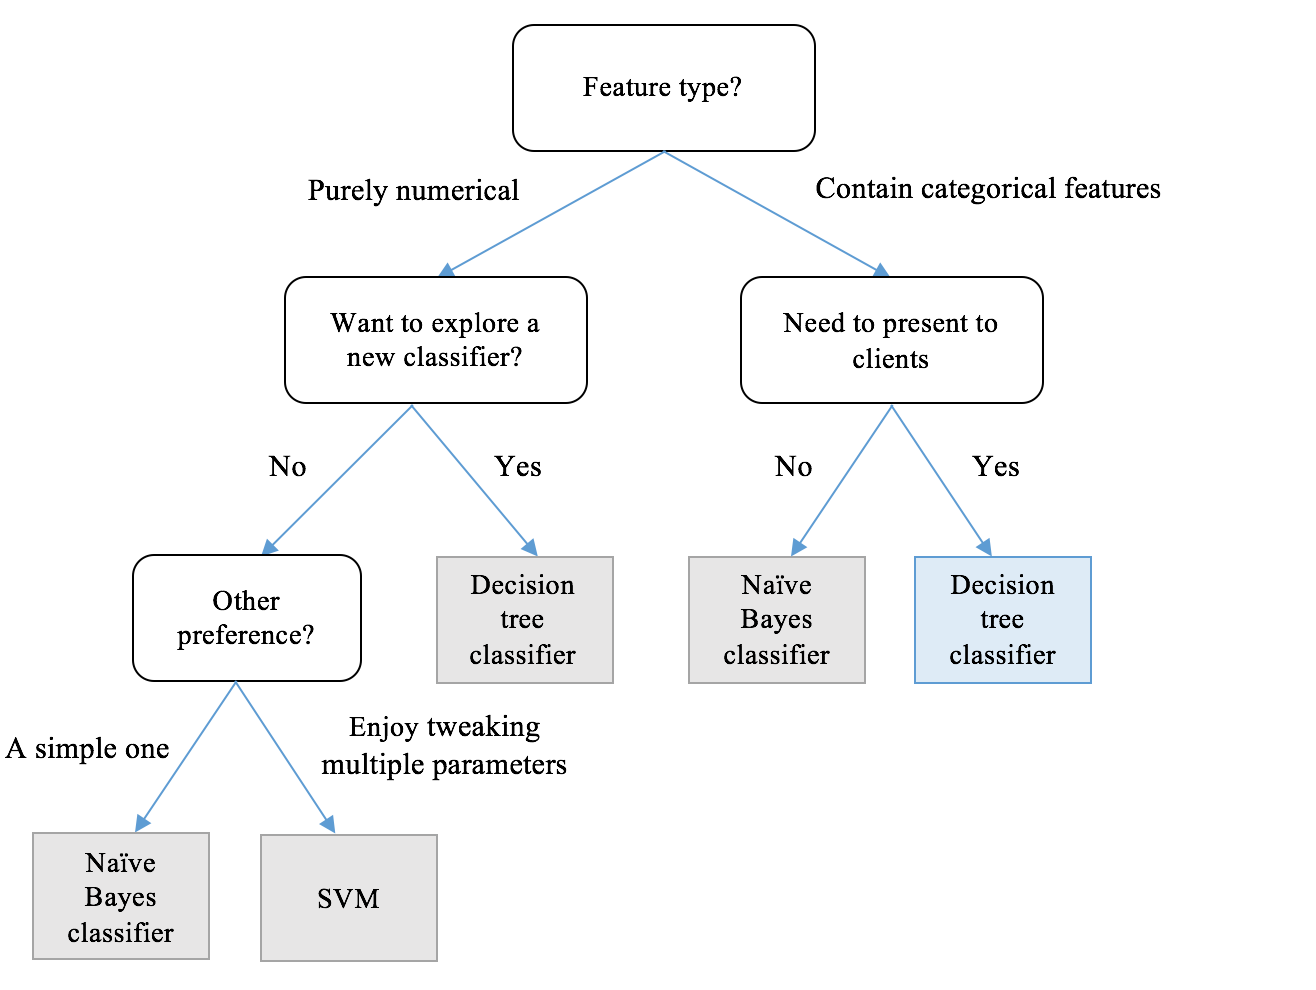
\includegraphics[width=0.9\textwidth]{metatree.png}
\end{frame}

\begin{frame}
\frametitle{Decision tree}
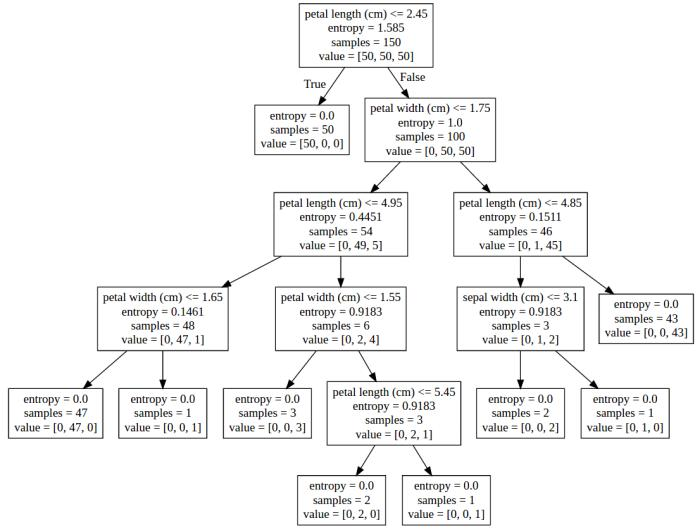
\includegraphics[width=0.9\textwidth]{bettertree.jpg}
\end{frame}


\begin{frame}
\frametitle{Constructing trees}

\begin{block}{Splitting rules}
The tree is constructed by selecting a feature and a value based on which we split the set of elements into two parts. This process is repeated with both subsets until some stopping criterion is fulfilled.
\end{block}

\begin{block}{Stopping criterion}
Examples: each subset contains only one class, the tree reach a certain depth, fewer misclassifications than a certain thresholds, next best feature for selection is worse than some threshold.
\end{block}
\end{frame}

\begin{frame}
\frametitle{Splitting rules}

\begin{block}{ID3}
We choose a feature with lowest entropy, e.g. a feature for which the information gain is the highest (mutual information with classes is the highest).
\end{block}

\begin{block}{C4.5}
Similar to ID3, but this time we optimize for highest normalized information gain. C4.5 can also work with numerical data.
\end{block}
\end{frame}


\begin{frame}
\frametitle{Splitting rules - 4th lab theory}

\begin{block}{Entropy}
$$H(Y) = \sum_{y \in \omega} - P(Y = y) \cdot log_2(P(Y=y))$$
\end{block}

\begin{block}{Specific conditional entropy}
$$H(Y| X = v) = H(Y), \textnormal{len pre hodnoty} Y, \textnormal{kde } X = x $$
\end{block}
\end{frame}


\begin{frame}
\frametitle{Splitting rules - 4th lab theory}
\begin{block}{Mutual information, information gain}
$$I(Y;X) = H(Y) - H(Y|X) = H(Y) - \sum_{x \in \omega} P(X = x)\cdot H(Y|X = x)$$
\end{block}

\begin{block}{Normalized information gain}
$$nI(Y;X) = \frac{I(Y;X)}{H(X)}$$
\end{block}
\end{frame}


\begin{frame}
\frametitle{Examples}

\begin{block}{ID3}
\url{https://sefiks.com/2017/11/20/a-step-by-step-id3-decision-tree-example/}
\end{block}

\begin{block}{C4.5}
\url{https://sefiks.com/2018/05/13/a-step-by-step-c4-5-decision-tree-example/}
\end{block}
\end{frame}


\begin{frame}
\frametitle{Matlab}
\begin{block}{fitctree}
Mdl = fitctree(X,y) - returns a tree classifier.
\end{block}

\begin{block}{fitctree}
Mdl = fitctree(T,property) - returns a tree classifier for table T and classification target in the property column of the table.
\end{block}

\begin{block}{CART}
Matlab uses the CART algorithm which is similar to ID3, but slightly different. It is not a part of the lecture so we will not deal with it now.
\end{block}
\end{frame}


\begin{frame}
\frametitle{Matlab}

\begin{block}{predict}
Mdl.predict(x) - returns model prediction
\end{block}

\begin{block}{view}
Mdl.view('Mode','graph') - displays the tree
\end{block}

\begin{block}{Exercise}
Create and display a tree for the fisheriris and census1994 database.
\end{block}
\end{frame}

\begin{frame}
\frametitle{Pruning the trees}
\begin{block}{Pruning}
The tree can be too complex which leads to overfitting. It is possible to prune the tree so that its subtrees which only provide marginal benefits are converted to leafs.
\end{block}

\begin{block}{prune}
MdlP = prune(Mdl,'Property', value) - returns a pruned tree based on the selected property.
\end{block}

\begin{block}{Exercise}
Prune the tree for the data in fisheriris and census 1994. Test various properties. Check if pruning helps the accuracy on the test set of census1994.
\end{block}

\end{frame}




\end{document}